%% Prof. Ed Merkle, University of Missouri
%% Charlie Redmon, University of Kansas
%% 20170918
%% SEM path diagram

% standalone class for individual image to be included in a document
% border=15pt controls the whitespace padding around the diagram
\documentclass[border=15pt]{standalone}

% load custom style configurations from separate file
%% ------------------------------------------------------------
%% Charlie Redmon
%% 20170923
%% semTikzStyle.tex: style configurations for SEM path diagrams
%% ------------------------------------------------------------

\usepackage{tikz}

% observed variable
\tikzstyle{ov}=[shape=rectangle,
                draw=black!80,
                minimum height=0.6cm,
                minimum width=0.6cm,
                thick]

% response variable
\tikzstyle{av}=[shape=rectangle,
                draw=black!80,
                fill=black!10,
                minimum height=0.6cm,
                minimum width=0.6cm,
                thick]

% latent variable
\tikzstyle{lv}=[shape=circle,
                draw=black!80,
                thick,
                minimum width=1cm]

% correlations
\tikzstyle{lcor}=[bend left=30, dashed]
\tikzstyle{rcor}=[bend right=30, dashed]

% self-loops (for variance)
\tikzstyle{lloop}=[loop left, 
                   out=210, 
                   in=150, 
                   distance=0.3cm,
                   densely dotted]

\tikzstyle{rloop}=[loop right, 
                   out=30, 
                   in=-30, 
                   distance=0.3cm,
                   densely dotted]

\tikzstyle{aloop}=[loop above, 
                   out=60, 
                   in=120, 
                   distance=0.3cm,
                   densely dotted]

\tikzstyle{bloop}=[loop below, 
                   out=-60, 
                   in=-120, 
                   distance=0.3cm,
                   densely dotted]




\begin{document}

%% ">=stealth" sets the arrow head style
%% "semithick" sets the line width (0.6 pt)
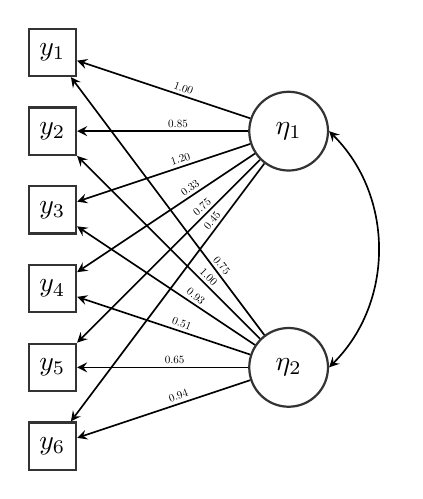
\begin{tikzpicture}[>=stealth,semithick]

% observed variables
\node[ov] (y1) at (0,-1)      {$y_1$};
\node[ov] (y2) [below of=y1]  {$y_2$};
\node[ov] (y3) [below of=y2]  {$y_3$};
\node[ov] (y4) [below of=y3]  {$y_4$};
\node[ov] (y5) [below of=y4]  {$y_5$};
\node[ov] (y6) [below of=y5]  {$y_6$};

% latent variables
\node[lv] (f1) at (3, -2)  {$\eta_1$};
\node[lv] (f2) at (3, -5)  {$\eta_2$};

% paths with loadings (rotated to align with path)
\path[->] (f1) edge node[above,pos=0.4,scale=0.4, rotate=-20] {1.00} (y1)
          (f1) edge node[above,pos=0.41,scale=0.4] {0.85} (y2)
          (f1) edge node[above,pos=0.39, scale=0.4, rotate=17] {1.20} (y3)
          (f1) edge node[above,pos=0.34,scale=0.4, rotate=35] {0.33} (y4)
          (f1) edge node[above,pos=0.29,scale=0.4, rotate=40] {0.75} (y5)
          (f1) edge node[above,pos=0.24,scale=0.4, rotate=50] {0.45} (y6)
          (f2) edge node[above,pos=0.25,scale=0.4, rotate=-50] {0.75} (y1)
          (f2) edge node[above,pos=0.31,scale=0.4, rotate=-45] {1.00} (y2)
          (f2) edge node[above,pos=0.36,scale=0.4, rotate=-40] {0.93} (y3)
          (f2) edge node[above,pos=0.41,scale=0.4, rotate=-20] {0.51} (y4)
          (f2) edge node[above,pos=0.43,scale=0.4] {0.65} (y5)
          (f2) edge node[above,pos=0.4,scale=0.4, rotate=20] {0.94} (y6);

% path between latent variables
\path[<->] (f1.east) edge [bend left=45] node[left,scale=0.8] {} (f2.east);

\end{tikzpicture}


\end{document}